%%&program=xelatex
%&encoding=UTF-8 Unicode
% SVN keywords
% $Author: bernardo $
% $Date: 2014-10-24 15:26:00 +0100 (Fri, 24 Oct 2014) $
% $Revision: 6732 $
% $URL: http://metis.ipfn.ist.utl.pt:8888/svn/cdaq/Users/Bernardo/Aulas/LFEB/teXfiles/ContrucoesGeometrica/ConstrucoesGeomet.tex $
\documentclass[a4paper,12pt]{article}      % Comments after  % are ignored
%\usepackage{hyperref}                 % For creating hyperlinks in cross references
%
%MUDAR procedimento lente divergente + angulo de Brewster
\usepackage{ifxetex}% for XELATEX, or PDFlatex
\usepackage{ifplatform} 
\usepackage{pst-optic} 
\usepackage{pstricks}
%
\ifxetex
	\usepackage{polyglossia} \setmainlanguage{portuges}
	\usepackage{fontspec}
	\ifwindows
		\setmainfont[Ligatures=TeX]{Garamond}
		\setsansfont[Ligatures=TeX]{Gill Sans MT}
		\setmonofont{Consolas}		
%		\setmonofont[Scale=MatchLowercase]{Courier}
	\fi
	\iflinux
		\setmainfont[Ligatures=TeX]{Linux Libertine O}
		\setsansfont[Ligatures=TeX,Scale=MatchLowercase]{Linux Biolinum}
		\setmonofont[Scale=MatchLowercase]{Courier}
	\fi
	\ifmacosx
	% add settings
	% Use xelatex -no-shell ...
		\setmainfont[Ligatures=TeX]{Garamond}
		\setsansfont[Ligatures=TeX]{Helvetica}
		\setmonofont{Consolas}
	\fi
	\usepackage{xcolor,graphicx} 
\else
	\usepackage[portuguese]{babel}
	%\usepackage[latin1]{inputenc}
	\usepackage[utf8]{inputenc}
	\usepackage[T1]{fontenc}
	\usepackage{graphics}                 % Packages to allow inclusion of graphics
	\usepackage{color}                    % For creating coloured text and background
\fi

\usepackage{enumitem}
\setlist{nolistsep}

\usepackage{tikz}
%\usetikzlibrary{calc,arrows,decorations.pathmorphing,intersections}


\usepackage{amsmath,amssymb,amsfonts} % Typical maths resource packages
\usepackage[retainorgcmds]{IEEEtrantools}

\oddsidemargin 0cm
\evensidemargin 0cm

\pagestyle{myheadings}         % Option to put page headers
                               % Needed \documentclass[a4paper,twoside]{article}
\markboth{{\small \it  Laboratório de Física Experimental Básica}}
{{\small\it MEFT - 1º Sem. 2014/2015} }

\addtolength{\hoffset}{-0.5cm}
\addtolength{\textwidth}{2.5cm}
\addtolength{\topmargin}{-1.5cm}
\addtolength{\textheight}{3cm}

%\textwidth 15.5cm
%\topmargin -1.5cm
\setlength{\parindent}{0pt}
\setlength{\parskip}{1ex  plus  0.5ex  minus  0.2ex}
%\parindent 0.5cm
%\textheight 25cm
%\parskip 1mm


% Math macros
\newcommand{\ud}{\,\mathrm{d}} 
\newcommand{\HRule}{\rule{\linewidth}{0.5mm}}

\author{Prof. Bernardo B. Carvalho} 

%%%%, Bernardo Brotas Carvalho\\bernardo@ipfn.ist.utl.pt} 
\date{ Outubro 2012} 

\begin{document} 

	
\includegraphics[width=0.2\textwidth]{../logo-ist}%\\[1cm]  %%  Logo_IST_color

	\HRule \\[0.5cm]
	{ \huge \sf  \textsc{Ótica Geométrica}} \\[0.4cm] % \bfseries 
%	{ \huge \sf  \textsc{Construções Geométricas em Lentes Delgadas (aproximação paraxial)} }\\[0.4cm] % \bfseries 
	{ \large \bfseries Construções Geométricas em Lentes Delgadas (aproximação paraxial)}\\
%	{ \large \bfseries Procedimento Experimental}\\
	\HRule \\%[0.5cm]

\section{\sf Lei de Snell-Descartes}

\begin{figure}
	[!hb]  \centering 
	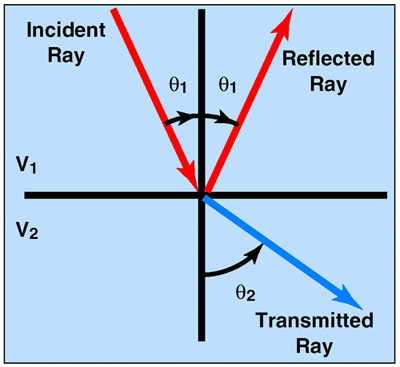
\includegraphics[width=0.4\textwidth]{snell}
%	\caption{. \label{fig:snell}} 
\end{figure}

 \begin{equation}
	\label{eq:snell}
	n_1 \cdot \sin \theta_1 = n_2 \cdot \sin \theta_2
\end{equation}

\section{\sf Construções Geométricas em Lentes Delgadas (aproximação paraxial}

\subsection{\sf Aproximações}

\subsubsection{\sf Lentes Delgadas}
Um Lente é considerada \textbf{delgada} quando a sua largura, $d$, é desprezavél façe à sua distância focal $d << f$.
\subsubsection{\sf Aproximação paraxial}
Feixes inclinados em relação ao eixo óptico de lente de um ângulo $\alpha$ , tal que
$\sin \alpha \approx \alpha$, e \\
 $\tan \alpha \approx \alpha\,$, com $\alpha < 0.1\,rad \sim 5^oº $

\begin{minipage}[c]{0.45\textwidth}
	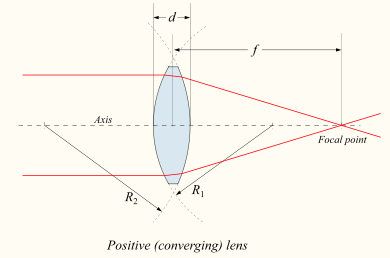
\includegraphics[width=\textwidth]{thinLens}
\end{minipage}
\begin{minipage}[c]{0.45\textwidth}
	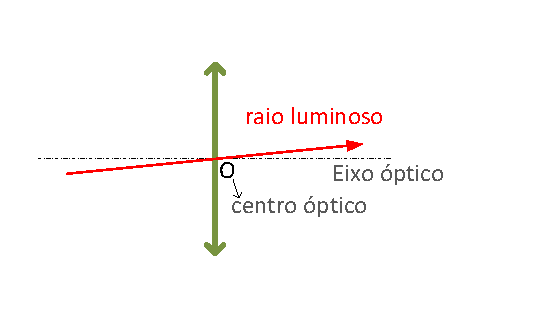
\includegraphics[width=\textwidth]{paraxial}
\end{minipage}

%\begin{figure}[!htb]  \centering 
%	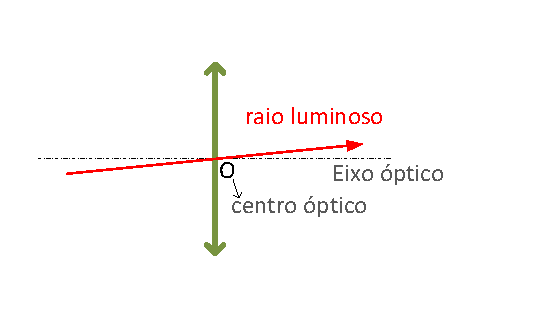
\includegraphics[width=0.7\textwidth]{paraxial}
%	\label{fig:paraxial}
%\end{figure}

\subsection{\sf Focos e Imagens}

%\begin{figure}	[!htb]  
{\centering 
	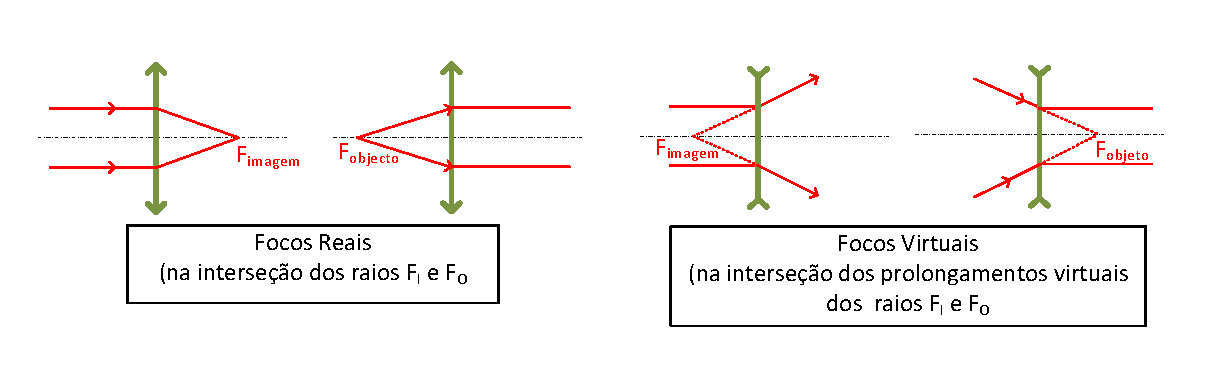
\includegraphics[width=\textwidth]{focoseImagem}
	}
%	\caption{. \label{fig:focoseImagem}} 
%\end{figure}

Nas imagens Reais o raios de luz passam de facto na posição da imagem e são as únicas que podem ser projetadas no ecrân. As imagens Virtuais, os raios parecem que vêm a imagem mas não passam nela e  são geralmente visíveis através da Lente.
\subsection{\sf Objeto e Imagem - Focos Conjugados}
Pela semelhança de triângulos.

\begin{pspicture}[showgrid=true](-7,-3)(7,3)
\rput(0,0){\lens[focus=2,OA=-3,AB=1,XO=0,YO=0,nameF=F_0,nameFi=F'_0,spotAi=0]}
\rput{0}(0,1.4){C}
\rput{0}(0,-2.4){D}
\rput{0}(4,-0.4){2F$_0$}
\rput{0}(-4,-0.4){2F$_0$}
\end{pspicture}

\begin{IEEEeqnarray}{rClrCl}
%\begin{array}{ccccc}
\Delta ABF_O \sim \Delta ODF_O  &\to & AB/A'B' = AF_O / F_O 0 &\to & AB/A'B' =  \frac{d_0-f}{ f} \label{eq:1} \\
\Delta ABO\sim \Delta A'B'O    &\to & AB/A'B' = AO / O A' &\to & AB/A'B' = d_O / d_I \label{eq:2} \\
\Delta COF_I \sim \Delta A'B'F_I  &\to & AB/A'B' = OF_I / F_I A' &\to & AB/A'B' =  \frac{f}{ d_I-f} \label{eq:3} 
\end{IEEEeqnarray}

de (\ref{eq:1}) e (\ref{eq:3}) obtemos a equação dos focos conjugados:
 
 \begin{equation}
	\label{eq:focosconjug}
    \fbox{
        $ \displaystyle
	\frac{1}{f} = \frac{1}{d_O} +\frac{1}{d_I} 
        $
    }
% \qquad \text{ equação dos focos conjugados}
\end{equation}



$AB$ e $A'B'$ são respetivamente as dimensões lineares transversais do objeto e da imagem  e define-se \textbf{ampliação transversal}, $A$:

$A =  \frac{A'B'}{ AB} $ que pode ser calculada por $A_{calc}=\frac{d_I}{d_O} $ atendendo a (\ref{eq:2})

No caso da última figura, $d_O > 0\;; \quad d_I > 0\,; \quad f > 0$ e a imagem é \textbf{real} e \textbf{invertida}.

\subsubsection{\sf Lente Convergente -  Imagem Real}
É fácil provar que para o funcionamento de uma máquina fotográfica  \fbox{$0 < A \le 1$ }:
(a imagem é posicionada no sensor da camera)

\begin{equation}
\infty > d_O \ge 2 f \quad \to \quad f > d_I \ge 2 f  
\end{equation}

e na montagem de um projetor de cinema ou de imagem de computador  \fbox{$1 \ge A < \infty$}:

\begin{equation}
f < d_O \le 2 f  \quad \to  \quad  2 f \le d_I < \infty 
\end{equation}

\subsubsection{\sf Lente Convergente - Imagem Virtual}

\subsubsection{\sf Funcionamento de uma Lupa}

\begin{figure}
	[!htb]  \centering 
	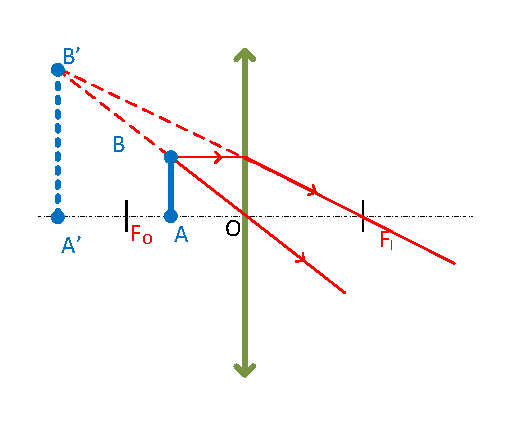
\includegraphics[width=0.8 \textwidth]{lupa}
%	\caption{. \label{fig:lupa}} 
\end{figure}

\begin{IEEEeqnarray}{rCl}
0 < d_O \le \frac{f}{2} \qquad & -f \le d_I < 0 \quad& -2 \le A < -1\\
\frac{f}{2} \le d_O < f \qquad& -\infty < d_I \le -f \quad& -\infty < A \le -2
\end{IEEEeqnarray}

\begin{pspicture}[showgrid=true](-7,-3)(7,3)
\rput(0,0){\lens[lensType=CVG,focus=4.5,OA=-2.7,AB=1,XO=0,YO=0,nameF=F_0,nameFi=F'_0,spotAi=0,drawing=true,rayColor=white]}
\psline[linecolor=red,linestyle=dashed](B')(F')
\psline[linecolor=red,linestyle=dashed](B')(B)
\psline[linecolor=red](B)(0,1)
\psline[linecolor=red](B)(2.7,-1)
\psline[linecolor=red](0,1)(F')
\psset{linecolor=red}
\Arrows[posStart=0,length=1](B)(0,1)
\Arrows[posStart=2,length=3](B)(0,0)
\Arrows[posStart=0,length=3](0,1)(F')
\rput(8,0){\psset{linecolor=black}\eye}
\end{pspicture}

\subsubsection{\sf Lente Divergente}
Para objetos reais a imagem é sempre virtual.


\begin{figure}
	[!htb]  \centering 
	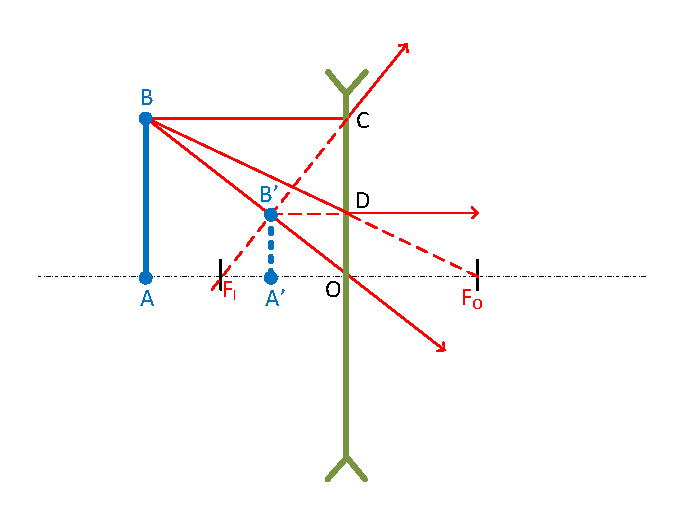
\includegraphics[width=0.8\textwidth]{diverg}
%	\caption{. \label{fig:lupa}} 
\end{figure}

\begin{center}
%\psscalebox{0.75}{
\begin{pspicture*}(-7.5,-3)(7.5,3)
	\rput(0,0){\lens[lensType=DVG,focus=-2,spotAi=270,spotBi=90]} %nameF=F_1,
	%\uput[270](A){A}
	%\uput[270](F){F}
	\uput[270](F'){$\mathrm{F'}$}
	\rput(8,0){\psset{linecolor=black}\eye}
	%}
\end{pspicture*}
\end{center}


$A'B'$ é uma imagem  \textbf{virtual}  e \textbf{direita} com $d_I <0$ (imagem do mesmo lado do objeto).
\begin{equation*}
f<0 \quad \to   d_O> 0 ; \quad  d_I <0  
\end{equation*}

A equação (\ref{eq:focosconjug}) pode ser obtida também pela semelhança de triângulos:

\begin{IEEEeqnarray}{rClrCl}
%\begin{array}{ccccc}
\Delta ABO \sim  \Delta A'B'O  & \to & AB/A'B' = \frac{d_0}{d_I} & \to & -\infty < A < 0 \label{eq:diver1} \\
\Delta ABF_0\sim \Delta DOF_O   &\to & \frac{d_0 + f}{f} = AB/A'B' & \to & \frac{d_0 + |f|}{|f|} = \frac{d_0 }{d_I}  \label{eq:diver2} \\
\Delta F_I C0 \sim \Delta F_I A'B'  &\to & \frac{|f|}{|f| - |d_I|} =AB/A'B'  &  \to &  \frac{|f|}{|f| - |d_I|} = \frac{d_0 }{|d_I|} 
\end{IEEEeqnarray}

As figuras construídas correspondem a objetos reais, i.e. são iluminados por luz proveniente da esquerda e 
situam-se antes da lente ($d_O > 0$).

\subsection{\sf Situação de Objetos Virtuais ($d_O<0$)}

\subsubsection{\sf Lente Convergente - Imagem Real}

\begin{minipage}[c]{0.6\textwidth}
%\begin{figure}
%	[!htb]  \centering 
	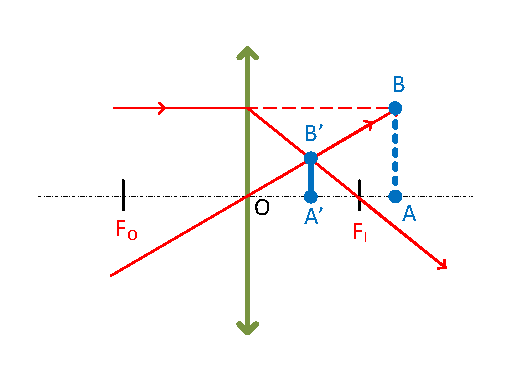
\includegraphics[width=\textwidth]{convergVirt}
%	\caption{. \label{fig:lupa}} 
%\end{figure}
\end{minipage}
\begin{minipage}[c]{0.4\textwidth}
Do objeto virtual obteve-se uma imagem \textbf{real} e \textbf{direita}.
\begin{IEEEeqnarray}{rCl}
 d_O < 0 ; \quad &&  f > 0   \nonumber\\
\frac{d_I}{-|d_O|}  & =&  \frac{f}{-|d_O| -f}     \nonumber
\end{IEEEeqnarray}
\end{minipage}

\subsubsection{\sf Lente Divergente - Imagem Virtual}

\begin{IEEEeqnarray}{rCl}
 d_O < 0 & &  f < 0   \nonumber\\
\frac{d_I}{-|d_O|}  & =&  \frac{|f|}{-|d_O| -|f|}     \nonumber
\end{IEEEeqnarray}

\begin{figure}
	[!htb]  \centering 
	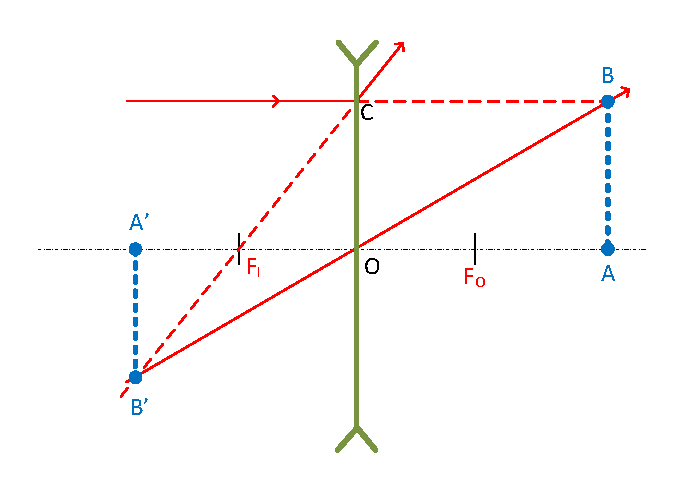
\includegraphics[width=0.7\textwidth]{divergVirt_I}
%	\caption{. \label{fig:lupa}} 
\end{figure}


Conclui-se que no caso de uma lente divergente com um objeto virtual que 
a imagem também é virtual e invertida: 
\begin{equation}
|d_O|  =  \left\{
\begin{array}{rl}
|d_O|   = |f|:  &   |d_I| \to \infty, \quad A \to \infty ,\\
|f| < |d_O|   < 2|f|:  &   |d_I|  <0 , \quad A  >1  ,\\
|d_O|   = 2|f|:  &   |d_I| = 2|f|, \quad A =1  ,\\
|d_O|  > 2|f|:   & |d_I|  <0 , \quad A  <1  .
\end{array}  \right.
%f<0 \quad \to   d_O> 0 ; \quad  d_I <0  
\end{equation}

\subsubsection{\sf Lente Divergente - Imagem Real}
\begin{IEEEeqnarray}{rCl}
\textrm{Se } d_O < 0 ; \quad  |d_O| <  |f|; \quad  |d_O| <  x|f| ; \quad (x < 1) & \to &    d_I >0; \quad A > 1 \nonumber
\end{IEEEeqnarray}


\begin{minipage}[c]{0.7\linewidth}
	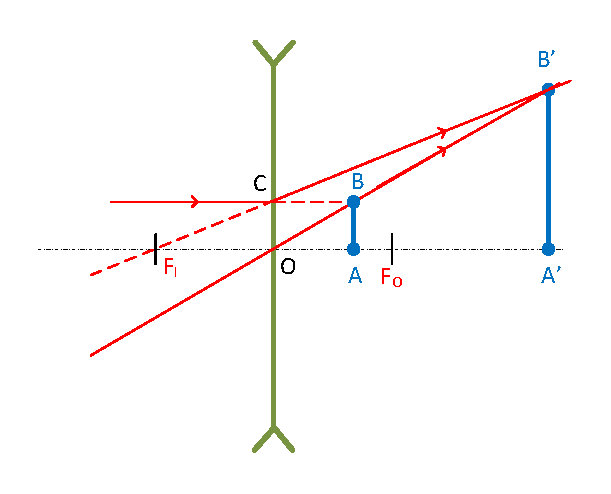
\includegraphics[width=0.7\textwidth]{divergReal}
\end{minipage}
\begin{minipage}[c]{0.3\linewidth}
A imagem é \textbf{real} e \textbf{direita}
\end{minipage}


\begin{pspicture*}(-7.5,-3)(7.5,3)
	\rput(0,0){\lens[lensGlass=true,lensWidth=0.5,lensType=DVG,XO=0,AB=2,OA=4,focus=6,spotAi=270,spotBi=90]%
 	\psline[linewidth=1pt](xLeft)(xRight)}
	\psline[linecolor=red,linestyle=dashed](I')(F)% Verlaengerung des Brennstrahls
	%\uput[270](F){F}
	\uput[270](F'){$\mathrm{F_O}$}
	%\psOutLine[length=7](B')(I){END}
	%\psBeforeLine[length=7](I')(B'){START}% permet de definir START
	%\pspolygon[style=rayuresJaunes,linestyle=none](B)(I)(END)(START)(I')
	%\psline(B)(I)(END) 
	%\psline(B)(I')(START)
\end{pspicture*}

%\begin{figure}	[!htb]  \centering 
%	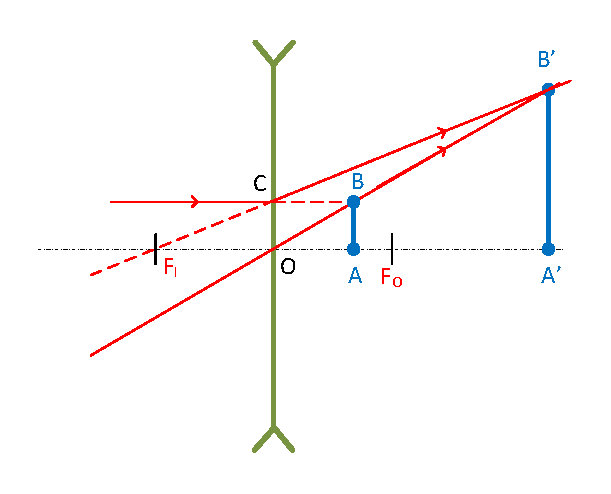
\includegraphics[width=\textwidth]{divergReal}
%	\caption{. \label{fig:lupa}} 
%\end{figure}

\subsection{\sf Associação de Lentes delgadas}

Para duas lentes delgadas de distâncias focais $f_1$ e $f_2$ afastadas de $D$ (para $D << f_1,f_2$) pode calcular-se a distância focal equivalente do conjunto através de: 

 \begin{equation}
	\label{eq:assoclentes}
    \fbox{
        $ \displaystyle
	\frac{1}{f_{equiv}} = \frac{1}{f_1} + \frac{1}{f_2} - \frac{D}{f_1 \,f_2} 
        $
    }
\end{equation}

A dificuldade, quando se usa o método direto quer dos focos conjugados, para a determinação da distância focal equivalente, ${f_{equiv}}$ é a medida das distâncias $d_O$ e $d_I$ 
(que são diferentes das distância do objeto e de imagem às superfícies das lentes ou ao seu planos médio.

É preferível usar a equação (\ref{eq:focosconjug}) para cada uma das lentes, e considerar que a primeira imagem (real ou virtual) irá constituir-se como o “objeto”  para a segunda lente. 

Vejamos o gráfico em diferentes posições.

\subsubsection{\sf Duas lentes Convergentes afastadas de $D$}
\begin{figure}	[!htb]  \centering 
	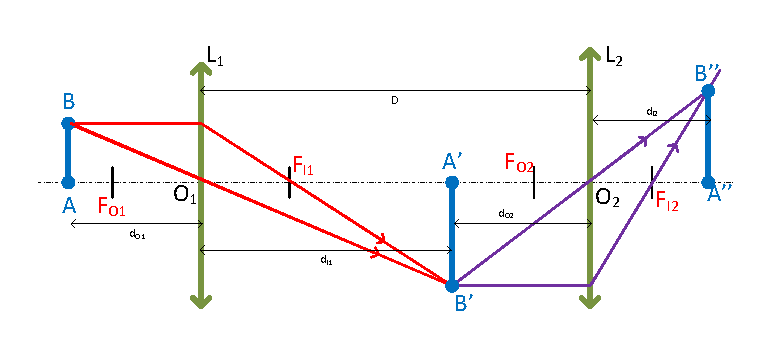
\includegraphics[width=\textwidth]{duplaConver_I}
%	\caption{. \label{fig:lupa}} 
\end{figure}

\begin{pspicture*}(-7.5,-2.75)(7.5,3)
	\rput(0,0){\lens[lensScale=0.6,XO=-4,nameF=F_1,nameA=A_1,nameB=B_1,
  		nameFi=F'_1,nameAi={ },nameBi={},nameO=O_1,focus=1,OA=-2,lensGlass=true, lensWidth=0.5]}
	%\pspolygon[style=rayuresJaunes,linestyle=none](B)(I)(B')(I')(B)
	\Transform
	\rput(0,0){\lens[lensScale=1.2,XO=2,focus=2,nameA=A'_1,spotA=90,nameB=B'_1,spotB=270,
  		nameO=O_2,nameAi=A'',spotAi=270,nameBi=B'',spotBi=90,nameF=F_2,nameFi=F'_2,
  		lensTwo=true,lensGlass=true,lensWidth=0.5]}
	%\pspolygon[style=rayuresJaunes,linestyle=none](B)(I)(B')(I')(B)
\end{pspicture*}

\begin{equation}
|d_O|  =  \left\{
\begin{array}{llll}
 \frac{1}{d_{O_1}} +  \frac{1}{d_{I_1}}   = \frac{1}{f_1}  & d_{O_1} = AO_1 & d_{I_1} = O_1A' & f_1 = O_1 F_{O_1} = O_1\,F_{I_1} ,\\
 \frac{1}{d_{O_2}} +  \frac{1}{d_{I_2}}   = \frac{1}{f_2}  & d_{O_2} = A'O_2 & d_{I_2} = O_2\,A'' & f_2 =  F_{O_2}\,O_2\, = O_2\,F_{I_2}, \\
O_1\,O_2 = D = d_{I_1} + d_{O_2}.
\end{array}  \right.
\label{eq:assoclentes_2}
\end{equation}

Esta é a montagem mais simples de um \textbf{telescópio}, a partir do qual se podem obter grandes ampliações.
Estas 3 expressões permitem calcular $f_2$, conhecidos os valores de $f_1$, $d_{O_1}$, $d_{I_2}$ e $D$.

No caso de uma imagem obtida por a uma lente, $L_1$, que passa a ser um “objeto” virtual para $L_2$.
\begin{figure}	[!htb]  \centering 
	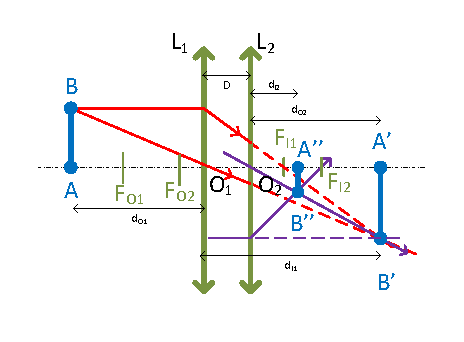
\includegraphics[width=0.8\textwidth]{duplaConver_II}
\end{figure}

\newpage
\subsubsection{\sf Lentes Convergente e Divergente afastadas de $D$}

\begin{figure}	[!htb]  \centering 
	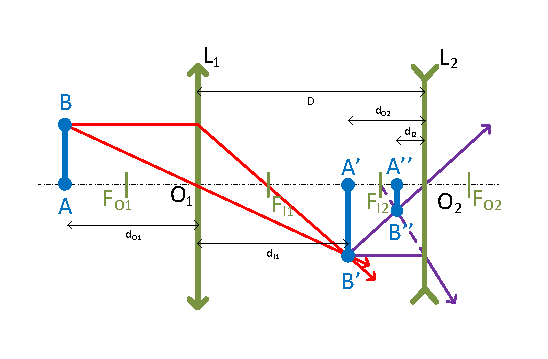
\includegraphics[width=0.8\textwidth]{ConverDiverg_I}
%	\caption{. \label{fig:lupa}} 
\end{figure}

Obtém-se uma imagem virtual produzida pela lente $L_2$ divergente a partir de imagem real obtida a partir da lente $L_1$

Na figura seguinte obtém-se uma imagem real $A''\,B''$ produzida pela lente $L_2$ divergente a partir de imagem  obtida a partir da lente $L_1$, que sua vez é um objeto virtual para a lente $L_2$

%\begin{figure}	[!htb] 
\begin{center}
	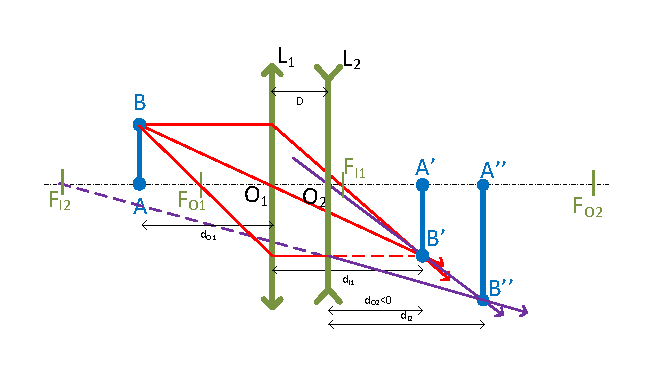
\includegraphics[width=0.8\textwidth]{ConverDiverg_II}
\end{center}

%	\caption{. \label{fig:lupa}} 
%\end{figure}


Se as lentes permutarem (Figura seguinte) obtem-se também uma imagem real  $A''\,B''$ se a distância $A\,O_1$ for semalhante nos 2 casos.
Em qualquer destas situações pode sempre calcular-se $f_2 < 0$ usando o conjunto das 3 equações (\ref{eq:assoclentes_2})

%\begin{figure}	[!htb]  
\begin{center}
	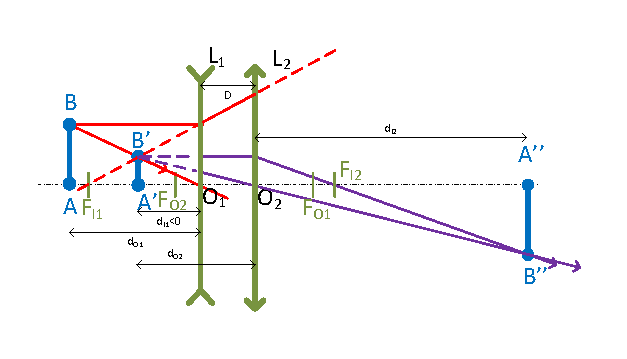
\includegraphics[width=0.8\textwidth]{ConverDiverg_III}
\end{center}
%	\caption{. \label{fig:ConverDiverg_III}} 
%\end{figure}

\clearpage
\section{Microscópio}

%\begin{LTXexample}
\begin{pspicture}(-7.5,-5.5)(7.5,3)
\rput(0,0){\lens[focus=1.5,OA=-2,AB=0.5,XO=-5,lensGlass=true,lensWidth=0.4,
   yBottom=-4,yTop=4,drawing=false,lensScale=0.4,nameF=F_1,nameFi=F'_1]
  \psline[linewidth=1pt](xLeft)(xRight)}
\pnode(! XO 1){UPlens1} \pnode(! XO -1){DOWNlens1}
\Transform
\rput(0,0){\lens[focus=2,XO=3,lensGlass=true,lensWidth=0.4,yBottom=-4,yTop=4,drawing=false,
        nameF=F_2,nameFi=F'_2,spotF=90,spotFi=90]}
\psline{->}(A1)(B1)\psline{->}(A'1)(B'1)\uput[270](A1){A}\uput[90](B1){B}
\uput[270](B'1){$\mathrm{B_1}$}\uput{0.7}[90](A'1){$\mathrm{A_1}$}
{\psset{linecolor=red}
 \rayInterLens(I11)(B'1){3}{Inter1L2}\rayInterLens(B1)(O1){3}{Inter2L2}
 \rayInterLens(UPlens1)(B'1){3}{Inter3L2}\rayInterLens(DOWNlens1)(B'1){3}{Inter4L2}
 \psline(B1)(I11)(B'1)(Inter1L2)\psline(B1)(Inter2L2)\psline(B1)(UPlens1)(Inter3L2)
 \psline(B1)(DOWNlens1)(Inter4L2)
 \psset{length=5}
 \Parallel(B'1)(O)(Inter3L2){B1inftyRigth}\Parallel(B'1)(O)(Inter4L2){B2inftyRigth}
 \Parallel(B'1)(O)(Inter2L2){B3inftyRigth}\Parallel(B'1)(O)(Inter1L2){B3inftyRigth}
 {\psset{length=-5,linestyle=dashed}
  \Parallel(B'1)(O)(Inter3L2){B1inftyLeft}\Parallel(B'1)(O)(Inter4L2){B2inftyLeft}
  \Parallel(B'1)(O)(Inter2L2){B3inftyLeft}\Parallel(B'1)(O)(Inter1L2){B3inftyLeft}
  \pcline[nodesep=6](B'1)(O)}
 \pspolygon[style=rayuresJaunes,linestyle=none](B1)(UPlens1)(Inter3L2)%
 	(B1inftyRigth)(B2inftyRigth)(Inter4L2)(DOWNlens1)
 \psline(B1)(UPlens1)(Inter3L2)(B1inftyRigth)\psline(B2inftyRigth)(Inter4L2)(DOWNlens1)(B1)}
\rput(7,0){\eye}
\end{pspicture}%


\newpage
\section{\sf Protocolo Experimental}

\subsection{\sf Questões a responder ANTES da sessão de Laboratório:}
\begin{enumerate}
\item Descreva por palavras suas quais os objectivos do Trabalho que irá realizar na sessão de Laboratório (uma folha A4). Indique as expressões que irá utilizar para obter as grandezas experimentais, bem como as expressões para calcular as incertezas. Inclua esta parte também no Relatório. Este irá constituir o ÚNICO meio de consulta na Prova Individual.
	
\item Utilizando uns óculos graduados (se não usar, peça a um colega), obtenha e registe a sua graduação. Calcule a distância focal, $f=1/Dioptrias$ (para miopia são lentes divergentes, para hipermetropia são convergentes. Ignore  a correção do astigmatismo).
\item Classifique as imagens visualizadas através das lentes, i.e: Reais/Virtuais, Direitas/Invertidas, Ampliadas/Reduzidas, Posição da Imagem relativa aos objetos.
\item Para uma lente de $-2.5$ Dioptrias calcule a posicão da imagem para um objeto a 40 cm da lente. A que distância está do objeto?
\item Para uma lente convergente (óculos ou uma lupa) em que condições obtém uma imagem virtual: a) direita; b) invertida?
\end{enumerate}

\subsection{\sf Material utilizado}
Caixa de Óptica equipada com calha graduada, lentes convergentes e divergente, semi-cilindro de 
vidro acrílico, diafragmas, polaroides, suportes. 
Fonte luminosa com lâmpada de incandescência linear. 

\subsection{\sf Procedimento Experimental}

\subsubsection{\sf  Índice de refracção dum vidro acrílico }

\begin{enumerate}
\item Utilizando a  fonte  luminosa  obtenha  um  feixe  de  luz  branca  de  raios  paralelos. Que tipo de lente necessita?
\item Com os diafragmas obtenha um feixe de luz estreito ($\approx 1\,mm$), alinhado com o eixo do Transferidor.
\item Faça  incidir  luz  branca  na  superfície  plana  do  semi-cilindro  de  vidro  acrílico.  Observe  e obtenha os ângulos de 
reflexão e a transmissão para vários ângulos do feixe incidente, à 
esquerda e à direita.  Faça  medições  pelo  menos  para  nove  valores  diferentes  do 
ângulo de incidência.
\item  Determine a) \emph{a partir do gráfico}, e b) por ajuste, o índice de refracção do vidro acrílico.  
\item Repita  as  medidas  e  a  análise  dos  resultados  fazendo  agora  a  incidência  na  superfície cilíndrica. 
\item  Compare o índice de refracção do vidro acrílico a partir da incidência nas duas faces. 
\item Estime também o valor do índice de refracção a partir do ângulo limite de reflexão total. 
\item  Compare a precisão dos diferentes valores obtidos de $n_{vidro}$. 
\end{enumerate}
	
\subsubsection{\sf Polarização da luz. Ângulo de Brewster}
Observe o efeito de interposição de dois polaroides paralelos ou cruzados no percurso de um feixe luminoso. 
Usando a mesma montagem do ponto anterior, polarize o feixe  paralelamente ao plano
de incidência. Para valores do ângulo de incidência próximos 
do  ângulo  de  Brewster  (que  pode  calcular  a  partir  dos  indice de refração) obtenha   o  intervalo 
angular em que extingue praticamente  do feixe refletido. 

\subsubsection{\sf   Distância focal de uma lente convergente ( $f  \approx 75\, mm$ ) }
 
\begin{enumerate}
\item Obtenha  um  feixe  de  luz  branca  de  raios  paralelos.
Determine  a  distância  focal (d.f.)  da  lente pelo método direto.  Repita  a  experiência  duas  vezes,  colocando  a  lente 
noutra posição relativamente à lente de raios paralelos. 
\item Coloque o \emph{objeto} com mira no suporte da calha, iluminado-o diretamente com a fonte luminosa. Coloque a mesma lente convergente a uma distância $150\,mm < d_O < 75 \,mm$ do objeto.

\item Com o ecrân plano procure a posição correta para obter uma \emph{imagem} focada.
Utilizando a equação dos focos conjugados, calcule de novo a d.f. da lente. 
\item Na folha quadriculada em anexo desenhe um diagrama com o eixo ótico, o objeto e a lente convergente. Utilizando as aproximações paraxial e das lentes delgadas desenhe a construção geométrica e obtenha a posição da imagem e a respetiva ampliação.

\item Medindo agora a imagem determine a ampliação linear. Compare-a com a que podia  calcular pelas distância $d_O$  e $d_I$. 
\item Repita a experiência duas vezes, colocando a lente noutras posições relativamente ao objeto.  
\item Compare o valor da distância focal com o obtido em a) e estime a precisão envolvida em 
cada um dos métodos que utilizou. 
\end{enumerate}
	
\subsubsection{\sf   Distância focal de uma lente divergente ( $f  \approx   -150\, mm$ ) }
\begin{enumerate}
\item Associe  no  mesmo  suporte  a  lente  divergente  com  uma  convergente ($f  \approx 75\, mm$) de  forma  que  o 
conjunto se comporte como um sistema convergente.
\item Repita a montagem com objecto e a sua imagem real. 
\item Conhecidas  a  distância  focal  da  lente  convergente  e  a  distância  entre  lentes, $D$, calcule  a 
distância focal da lente divergente a partir de $d_O$  e $d_I$. 
\item Repita a experiência (pelo menos uma vez), colocando o conjunto das lentes noutra posição 
relativamente ao objeto. 


\end{enumerate}
	
\newpage
\def\width{18}
\def\hauteur{25}
\begin{tikzpicture}[x=1cm, y=1cm, semitransparent]
\draw[step=1mm, line width=0.1mm, black!30!white] (0,0) grid (\width,\hauteur);
\draw[step=5mm, line width=0.2mm, black!40!white] (0,0) grid (\width,\hauteur);
\draw[step=5cm, line width=0.5mm, black!50!white] (0,0) grid (\width,\hauteur);
\draw[step=1cm, line width=0.3mm, black!90!white] (0,0) grid (\width,\hauteur);
\end{tikzpicture}


\end{document} 